\section{Text Editors}
When editing files on the Raspberry Pi there are multiple options, depending on whether you choose to edit the file in a specific program, or edit it within the command shell.

\subsection{GUI Based Text Editors}
\subsubsection{Notepad++}
Notepad++ is a text editor for Windows. It can be downloaded \href{https://notepad-plus-plus.org/download}{here}. Language can be set to enable syntax highlighting. To ensure you use spaces instead of tabs, go to Settings - Preferences - Tab Settings - tick the box "Replace by Space"..

\begin{figure}[H]
\centering
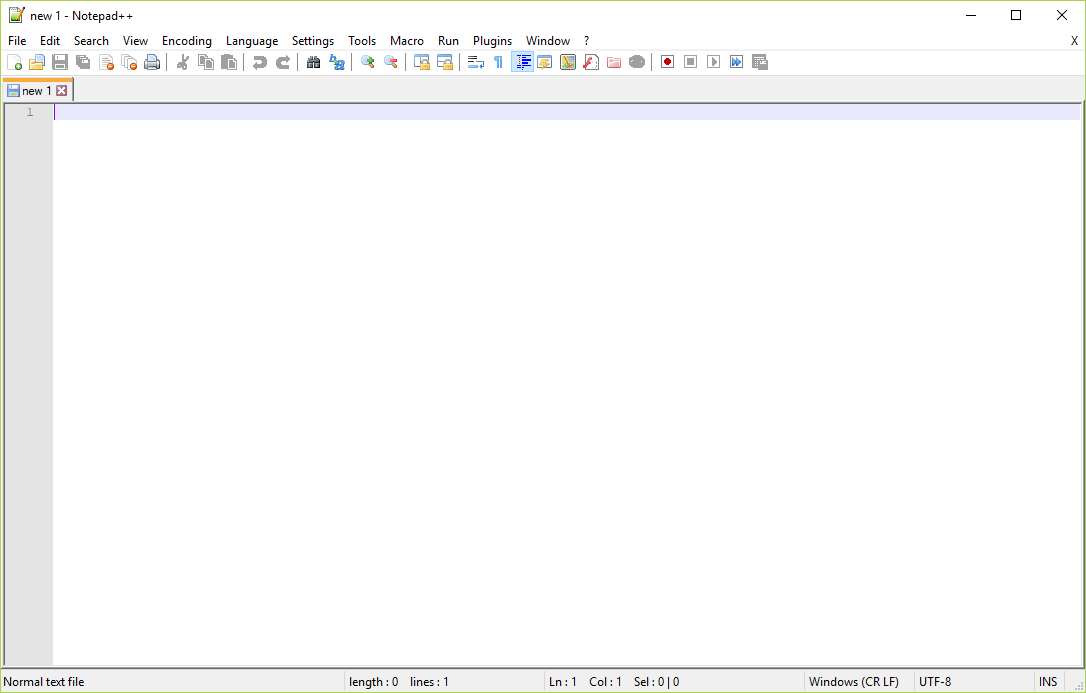
\includegraphics[width=0.6\columnwidth]{Figures/notepad++}
\caption{The Notepad++ text Editor}
\label{fig:notepad++}
\end{figure}

\subsubsection{Geany}
Geany is a GUI based text editor for Linux. It is very similar to Notepad++ on Windows and supports essentially the same features. The programming language can be set for syntax highlighting. Take note of whether you are using tabs or spaces (4 spaces is recommended for indentation). This can be set through preferences - editor - indentation - type - spaces. After changing the setting, close and reopen the file.

\begin{figure}[H]
\centering
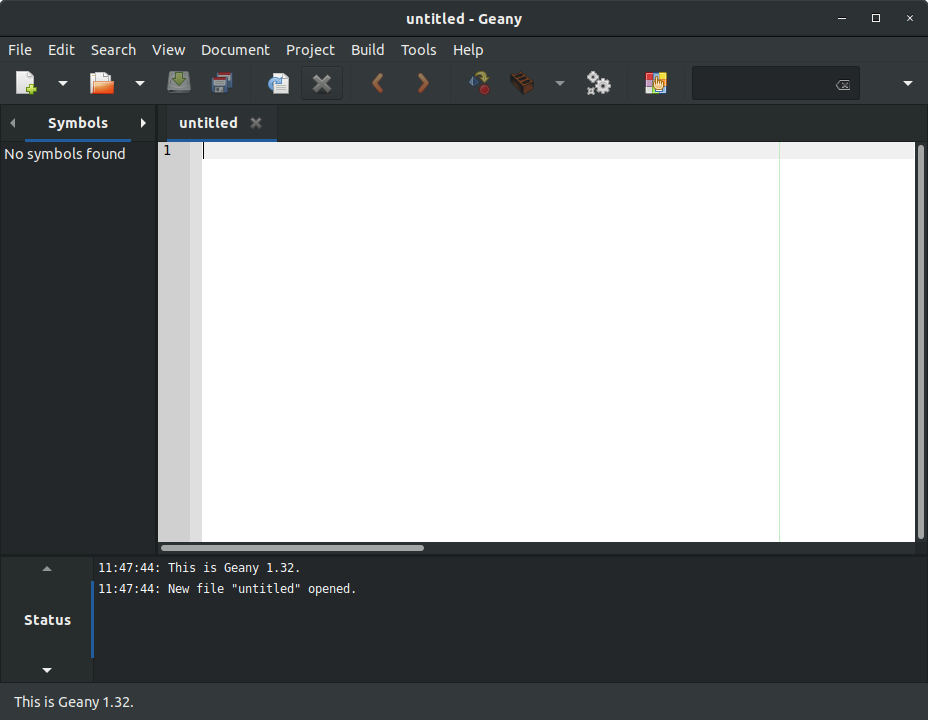
\includegraphics[width=0.6\columnwidth]{Figures/Geany}
\caption{The Geany Text Editor}
\label{fig:geany}
\end{figure}


\subsection{Terminal Based Text Editors}
\subsubsection{Nano}
Nano is a very easy to use file editor that runs within the command shell. Nano comes installed on Ubuntu and Raspbian by default, but if you do find yourself needing to install it, you can run
\begin{lstlisting}
$ sudo apt-get install nano
\end{lstlisting}

Once it is installed, you can use nano to edit text files by typing
\begin{lstlisting}
$ nano filename
\end{lstlisting}

You will be presented with an interface like this (currently the user is editing the python template):
\begin{figure}[H]
\centering
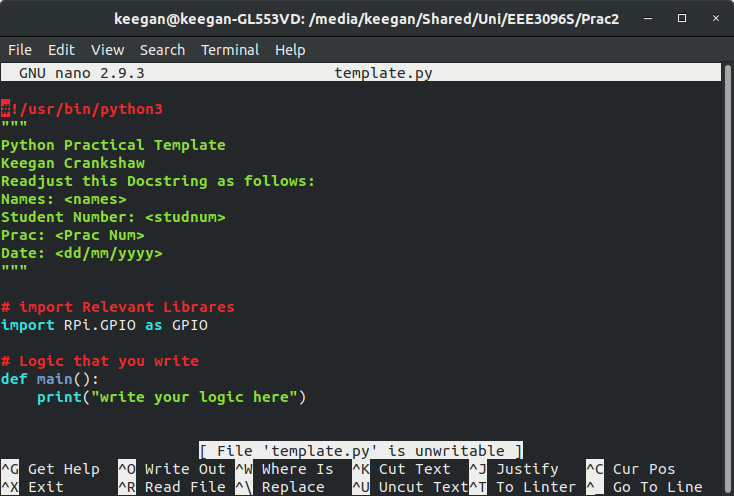
\includegraphics[width=0.6\columnwidth]{Figures/nanooutput}
\caption{The python template opened in nano}
\label{fig:nanooutput}
\end{figure}

Commands for nano are displayed on the bottom. A quick reference is as follows:
\begin{itemize}
\item Arrow Keys to move around as expected
\item Ctrl-W to find (Where is)
\item Ctrl-O to save (Write Out)
\item Ctrl-X to Exit (will be prompted to save on exit, press 'y' to save, press 'n' to exit without saving)
\item On Windows using Putty SSH client, 'paste' is performed by right-clicking with the mouse anywhere in the window, the contents of the clipboard will be pasted at the current cursor location
\end{itemize}

Note: By default, nano inserts a tab when the tab key is pressed. If you'd like to change this to insert a number of spaces, for example, four (as is \href{https://www.python.org/dev/peps/pep-0008/#tabs-or-spaces}{recommended by PEP 8}), do the following:
\begin{itemize}
\item Edit your ~/.nanorc file (or create it)
\begin{lstlisting}
$ sudo nano ~/.nanorc
\end{lstlisting}
\item Edit it to contain the following:
\begin{lstlisting}
set tabsize 4
set tabstospaces
\end{lstlisting}
\item Reboot your Pi to enable the changes
\end{itemize}

\subsubsection{Other Terminal Editors}
There are other terminal based text editors, such as emacs and vim. Feel free to use whichever you are comfortable with.

